\documentclass{article}
\usepackage[utf8]{inputenc}
\usepackage[T1]{fontenc}
\usepackage{lmodern,textcomp}
\usepackage[frenchb]{babel}
\usepackage{amsmath,amsfonts}
\usepackage{graphicx}
\title{Machine Learning - Lesson n°11}
\author{Chloé-Agathe Azencott}
\date{December 2016}
\DeclareMathOperator*{\argmax}{arg\,max}
\begin{document}

\maketitle

Scribes : Rémi Lalanne, Adam Hotait and Devang Thakkar

\section{Introduction}
In Machine Learning, it appears necessary to reduce the dimensionality of data set. There are various reasons to do so :

\begin{itemize}
    \item Computational complexity : the goal is to reduce the computational cost in time and space and therefore to avoid data overfitting.
    
    \item Interpretability, so that models are easier to interpret by human users.
    
    \item To simplify the models and make them more robust since there is less variance.
    
    \item Data visualization : the goal is to make this visualization easier for a human, for instance doctors who want to visualize plenty of data of their patients.
    
    \item To curb the cost of data acquisition, that can be very high in some cases.
    
    \item To keep only relevant and non-redundant attributes, since irrelevant and redundant attributes can prevent the algorithm from being efficient.
    
\end{itemize}

\bigskip

\textbf{Feature selection and feature extraction} are two ways of accomplishing dimensionality reduction.

On the one hand, the idea of feature selection is to select $m<p$ features among the $p$ existing features, and to ignore the remaining $(p-m)$ features. There are three ways to proceed :
\begin{enumerate}
    \item \textbf{Filtering approaches} that calculate a feature relevance score thanks to a statistical measure. Low-scoring features are then removed. These methods have a low computational cost and are independent of the classification algorithm but each feature is considered separately, so they ignore features dependencies.
    
    \item \textbf{Wrapper approaches} that aim at finding the best set of features for a given predictive model but that can be computationally very expensive.
    
    \item \textbf{Embedded approaches} that simultaneously fit a model and learn which features should be included. They are specific to a model.
\end{enumerate}

All these approaches are supervised.

\bigskip
On the other hand, the idea of feature extraction is to project the $p$ features on $m<p$ new dimensions. There are several approaches, such as linear approaches (Principal Components Analysis, Factor Analysis, MultiDimensional Scaling), supervised approaches (Linear Discriminant Analysis), non linear approaches (Isometric feature mapping, Locally Linear Embedding, Autoencoders).


\section{Feature selection : subset selection}
In a feature subset selection problem, the issue is to select a subset of features, so that all the attention concerns this subset and that the rest can be ignored.


\subsection{Wrappers approaches}

The goal is to find the subset of features that leads to the best-performing algorithm, knowing that there are $2^p$ subsets of p features. Indeed, if we consider p features, each feature can be present or  absent in the remaining features, so there are two choices for each future, hence $2^p$ such sets at the end.
Therefore, it is almost impossible to search the whole space exhaustively, except in the cases where $n$ is very small, since complexity is $O(2^p)$.
\bigskip

To solve this problem, we can use a greedy approach ("algorithme glouton" in French) : the forward search.
We proceed  by adding the "best" feature at each step. Let $E(F)$ be the error on held-out validation set of a predictor trained only using the features in $F$.
\begin{itemize}

    \item Initially, $F = \emptyset $
    
    \item Then, we find a new best feature : $j*= arg \ min_{j \in \{1,...,p\}} E(F\cup \{j\})$
    
    \item If $E(F)<E(F \cup \{j\})$ : the algorithm stops.
    
    \item Else : $F \leftarrow F \cup \{j\}$.
    
\end{itemize}

The error is therefore minimal and the complexity is $O(p^2)$, which is way better than $O(2^p)$.


\subsection{Embedded approaches}
We have seen algorithms which simultaneously optimize a cost/loss function and the features that should be uses.
Among them, the $L1$ regularization, with an approach called the Lasso. For a parameter $\lambda \geq 0 $, this approach finds $\widehat{\beta}_{lasso} = arg \ min_{\beta} \| y-X\beta \|_{2}^{2} + \lambda \| \beta \|_2 $.

\section{Feature extraction : Principal Components Analysis}

Another way of reducing the dimensionality of the data is use to Principal Component Analysis. The primary objective that we need to achieve is the minimization of information loss after the data has been projected onto a lower dimensional space using a linear mapping. In other words, we need to find a lower dimensional space, where the variance of the projection is maximised.

\bigskip

A few things to be noted here are:
\begin{itemize}
    \item PCA is an unsupervised method, in the sense that when project our values, we only consider the data points without paying any heed to the labels that pertain to those points.
    \item In PCA, one of our early assumptions is that the data that we have is centred; that is to say, the mean of our data is 0.
    \item PCA is a variance maximising exercise, hence it requires the data to be normalized before we can apply it correctly.
\end{itemize}

\bigskip

\subsection{Finding the Principal Components}
The goal is to find a space which maximizes the variance of the data that is projected on it. Before we begin, we define a certain terms that would enable us to understand better the derivation process. Let $w$ be a unit vector on which we wish to project our matrix of data points $X$.
This would imply that the projection of $X$ in the direction $w$ is given by $z = w^T X$. The variance of $z$, as calculated in the slides, comes out to be $w^T(\Sigma)w$ where $\Sigma$ is the covariance of X under the assumptions of a centred dataset.

\subsubsection{Finding the first component}
We need to begin by finding a vector that maximizes the variance of the projection $z$ and has unit magnitude. A problem of this type takes the form of a Lagrangian optimisation that can be solved easily by introducing a Lagrangian multiplier. Putting it mathematically, the problem is transformed from $(1)$ to $(2)$:

\begin{gather}
    w_1 = \argmax_ { w \in R_p} Var(w^T x) \\
    w_1 = \argmax_ { w \in R_p} (w^T \Sigma w - \alpha (w^Tw \ - \ 1))
\end{gather}

As with any ordinary Lagrangian problem, we derive the resulting equation and set it to 0. Doing this leads us to a couple of astonishing results. We find out that:

\begin{itemize}
    \item The system has been reduced to an eigen value problem
    \item The multiplier $\alpha$ is an eigen value of the matrix $\Sigma$
    \item The direction vector $w_1$ is an eigen vector of the matrix $\Sigma$
\end{itemize}

Using this results, we find out that the desired direction vector is the eigen vector with the largest eigen value.

\subsubsection{Finding the remaining components}
Once we have the first principal component, we proceed to find the remaining components. The process is really similar to the previous case, except for the fact that we have one more condition on our vector $w_i$, that is, the new vector $w_i$ must be orthogonal to all the previously found components. This algorithm leads to the discovery that the $i^{th}$ component is the eigen vector with the $i^{th}$ largest eigen value.

\bigskip

Once we have all the principal components of the data, we can choose to keep the top $m$ components and discard the rest. An important variable to decide here is $m$, i.e., how many principal components do we retain. One way to decide is to plot a scree graph of the variance explained by the components and select as many variables as required as long as the addition of one more components seems useful to the total variance explained.

\section{Feature extraction : Autoencoders}

A third way to do dimensionality reduction is to use neural networks, with the use of Autoencoders. Autoencoders try to reconstruct its input. However, and that is where it uses neural networks, the interest of autoencoders is the hidden layer(s) it constructs. Autoencoders are a non linear, unsupervised approach to dimensionality reduction.

\subsection{General presentation}

The goal is to select fewer features than there are in the train set to then reconstruct the train set. This is done on several points of data to find the weights that minimize the reconstruction error.

\begin{figure}[!h]
    \center
    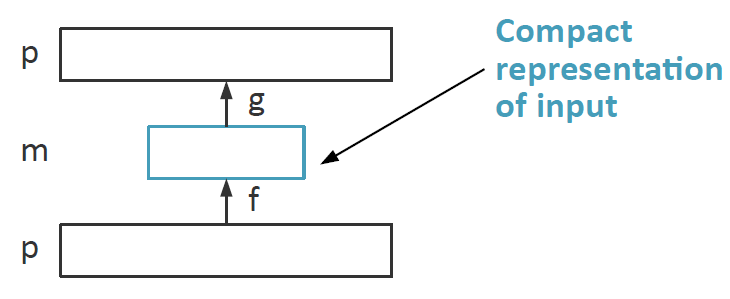
\includegraphics[scale=0.5]{./figures/autoencoder_general.png}
    \caption{Diagram of a generic autoencoder}
\end{figure}

\subsection{Restricted Boltzmann Machines}

RBM are stochastic neural networks, where the activation of a unit is probabilistic, with : \[P(o_i = 1) = \frac{1}{1+e^{-a_i+\sum_j o_j w_{ij}}}\]

\begin{figure}[!h]
    \center
    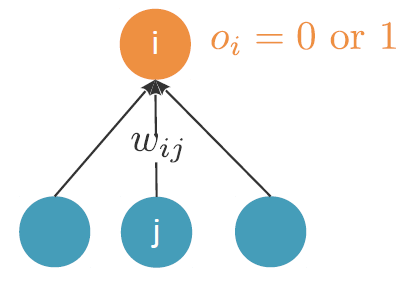
\includegraphics[scale=0.5]{./figures/autoencoder_stochastic.png}
    \caption{Diagram of a stochastic neural network}
\end{figure}

A RBM has two layers, with bidirectional connections. The term "restricted" comes from the fact that there are no connection between the hidden units.

The main property of a RBM is the energy of the RBM, defined by : \[E(\textbf{x},\textbf{z}) = - \sum\limits_{j=1}^p a_jx_j - \sum\limits_{h=1}^H b_hz_h - \sum\limits_{j=1}^p\sum\limits_{h=1}^H x_jw_{jh}z_h\]

where $a_j$ is the offset for the visible unit j and $b_h$ is the offset for the hidden unit h.

\begin{figure}[!h]
    \center
    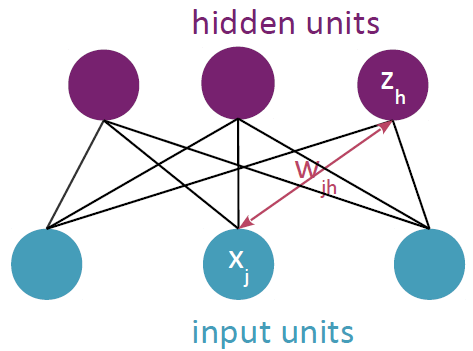
\includegraphics[scale=0.5]{./figures/autoencoder_rbm.png}
    \caption{Diagram of a RBM}
\end{figure}

The goal is to model the probability distribution $P(\textbf{x})$, with : \[P(\textbf{x}) = \frac{\exp(-\mathcal{F}(\textbf{x}))}{Z}\]

where $\mathcal{F}$ and $Z$ are respectively the free energy and the partition function (which is a normalizing factor), with :
\[ 
\left\{
  \begin{array}{rcc}
    \mathcal{F} & = & - \log\sum\limits_{\textbf{z}}\exp(-E(\textbf{x},\textbf{z})) = - \sum\limits_{j=1}^p a_jx_j - \sum\limits_{h=1}^H\log\sum\limits_{z_h}e^{z_h(b_h+\sum_{j=1}^pw_{jh}x_j)}\\
    Z & = & \sum\limits_{\textbf{x}\in\omega}\exp(\mathcal{F}(\textbf{x}))\\
  \end{array}
\right.
\]

\subsection{Deep architectures}
It should be noted that by stacking RBM (outputs of RBM become inputs for other subsequent RBM), we get Deep belief networks.

\begin{figure}[!h]
    \center
    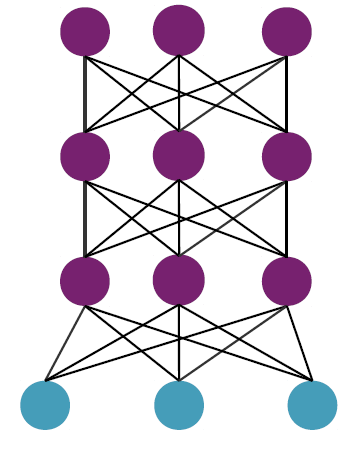
\includegraphics[scale=0.5]{./figures/autoencoder_deepbelief.png}
    \caption{Diagram of a deep belief network}
\end{figure}

\end{document}
